\documentclass[a4paper,oneside]{article}

%%%%%%%%%%%%%%%%%%%%%%%%%%%%%%%%%%%%%%%%%%%%%%%%%%%%%%%%%%%%%%%%%%%%%%%%%%%%%%%%%%%%%%%%%%%%%%%%%%%%%%%%%%%%%%%%%%%%%%%%%%%%%%%%%
%% PREAMBLE

% declare packages:

\usepackage{amsmath}
\usepackage{amsfonts,amsmath,amsthm}			% standard ams packgages
\usepackage[title,titletoc,toc]{appendix} % Appendix package. Not necessary, but it does make managing appendices easier
\usepackage{bm}										% bold maths symbols shorter definition: \bm{}
\usepackage{booktabs}							%	neat lines/rules for tables
\usepackage{eurosym} 							% neat symbols for Euro
\usepackage{float}								% allows more control over floats (figures, tables, etc.)
\usepackage{graphicx}							% for including graphics
\usepackage{lipsum} 							% insert random text (Lorem Ipsum)
\usepackage[colorlinks]{hyperref} % colorlinks colours the links instead of boxing them
\usepackage{natbib}								% references
\usepackage{setspace}							% single, 1.5, double spacing
\usepackage{url}									% like hyperref
\usepackage[euler]{textgreek}
\usepackage{rotating}
\usepackage{{xcolor}
\newcommand\myworries[1]{\textcolor{red}{#1}}
%%%% Make some adjustments to the document

% change from singlespace to onehalfspace to doublespace
%\singlespace
\doublespace
%\doublespace

% define title, author, etc.

\title{Cable Company Case Study}

\author{James Morgan}

\date{\today}

%% END OF PREAMBLE
%%%%%%%%%%%%%%%%%%%%%%%%%%%%%%%%%%%%%%%%%%%%%%%%%%%%%%%%%%%%%%%%%%%%%%%%%%%%%%%%%%%%%%%%%%%%%%%%%%%%%%%%%%%%%%%%%%%%%%%%%%%%%%%%%

\begin{document}

\maketitle

\begin{singlespacing} % wraps abstract to be written with single line spacing
	\begin{abstract}
		This paper focuses on the exorbitant cost and lack of quality of broadband internet access
		in the United States relative to OECD countries and the inefficient competitive
		dynamics present in the Cable Industry. More specifically, it shows that Cable Companies will
		not be able to compete in perpetuity due to innovation, inflation, higher interest rates and an
		excessive debt load. By utilizing a continuous state model of industry entry and exit, this paper
		highlights the unlikelihood that US Cable Companies will continue to have strong performance.
		Moreover, rising inflation and higher interest rates will present even stronger headwinds for
		Cable Companies. These findings will demonstrate the high social costs created by the Cable
		Companies and present a call to action for entrepreneurs and regulatory authorities.\end{abstract}
	\end{singlespacing}
\pagebreak

\section{Introduction}
	\:\:\:\:\:\: The shift to remote work has increased the need for network connectivity and is
	beginning to commoditize network services. Consequently, federal and state agencies have taken
	an interest in the industry. Moreover, alternative conduits for broadband connection present a
	market ripe for disruption through innovation. For example, Elon Musk's company Starlink may
	be able to offer more affordable internet access to customers in rural areas. Starlink uses
	advanced satellites in a low orbit to provide low latency broadband internet access across the
	globe. The development and implementation of 5G may further dampen Cable Company profits,
	especially since 20\% of Americans are smart phone only users. (Bandyopadhyay et al. 2020)

	The looming threat of an economic downturn is yet another headwind for Cable
	Companies. The CPI was up 5.4\% year over year in September and the threat of high long term
	inflation is very real. The COVID-19 pandemic and associated government support has created
	an extremely tight labor market. According to the NFIB, 51\% of small business owners reported
	job openings they could not fill in September 2021. This is a record high and is up one point
	from the previous month. (“Jobs Report and Jobs Data from the NFIB Small Business Research
	Center”, n.d.) It seems likely that the FED's hand will be forced and interest rates will rise as a
	function of inflation.

	The relative cost and quality of broadband internet access in the United States poses
	serious concerns about the efficacy of the industry model. The bar graph from the OECD
	Broadband Portal below indicates that the United States is behind many competitors regarding
	broadband internet penetration. This is surprising given the United States overall economic
	presence and brings to the light pressing need to increase penetration rates.

\section{Literature Review}

	This is a citation. ~\citep{Dixit_1989}

\section{Data}

\:\:\:\:\:\: The primary dataset for this project comes from the 2021 third quarter Charter Communications trending schedule.~\citep{chtr_rep} 
Charter Communications' business model is more focused on broadband internet and is, consequently, more suitable for this project.
Only revenues attributed to internet service are included in the project dataset. 
Furthermore, costs and expenses that are explicitly used for non-internet related activities are removed from the dataset.
In an abundance of caution, any costs and services that relate to internet services are included in the final dataset. 
It is assumed that these cost and expenses are required operating expenses for a purely broadband internet service company.
The final dataset is adjusted to a per customer level so that the model can test for markets of different sizes.
Additional information about financial calcuations is provided in the appendix.

\section{Models}
\subsection{Profit Model}
\:\:\:\:\:\: Consider a profit model for a cable company that is defined by internet revenue per passing less two costs bases: \emph{C\textsubscript{f}} and \emph{C\textsubscript{v}}. 
\emph{C\textsubscript{f}} represents the fixed average customer per customer and \emph{C\textsubscript{v}} represents the variable average cost per customer. 
Additional information about financial calcuations is provided in the appendix. 
\begin{equation}
	\pi_{t} = \emph{rev} * \emph{pen} - (C_{f}+C_{v})
\end{equation}
This equation represents the short run profit per quarter. 
Due to significantly high fixed costs, \emph{C\textsubscript{f}} is to be paid each period and theoretically, represents required interest payments.

Now consider a new cable company entering the market at time t\textsubscript{new}:
\begin{equation}
	\pi_{t_{new}} = \emph{rev} * \emph{pen} - (C_{f}+C_{v})
\end{equation}
Assuming all else equal, the fixed cost for the new cable company is adjusted to the new interest rate.

\subsection{Optimal Monetary Policy Model}

\:\:\:\:\:\:\:\:Consider a monetary authority who wishes to control the nominal interest rate  \emph{x} to minimize the variation of the inflation rate s\textsubscript{1} + the GDP gap s\textsubscript{2} around specified targets s\textsuperscript{*}\textsubscript{1} and s\textsuperscript{*}\textsubscript{1}.

\begin{equation}
	L(s) = 0.5(s-s^{*})^{T}\Omega(s-s^{*})
	\label{eq:mye1}
\end{equation} 
The corresponding state transition function is: 

\begin{equation}
	g(s,x,\epsilon) = \alpha + \beta \gamma x + \epsilon
	\label{eq:myeq2}
\end{equation} 

\begin{equation*}
s \subseteq \mathbb{R}^{2} \:\:\:	
x \subseteq [0, \infty)
\end{equation*}

Where s is a 2x1 vector containing the inflation rate and the GDP gap, s* is a 2x1 vector of targets, and Ω is a 2 x 2 constant positive definite matrix of preference weights. 
\begin{equation*} % stars * suppress labels / numbers appearing
	\bm{s^{*}} = 
		\left.
			\begin{bmatrix}
				0	\\
				1	\\
			\end{bmatrix}
		\right.
	\bm{\Omega} = 
		\left.
			\begin{bmatrix}
				0.3	&	0.0\\
				0.0	&	1.0\\
			\end{bmatrix}
		\right.
\end{equation*}

Assume that the inflation rate and the GDP gap are a joint controlled exogenous linear Markov process.

\begin{equation}
	s_{t+1}= \alpha+\beta s_{t}+\gamma x_{t}+\epsilon_{t+1} 
	\label{eq:mye3}
\end{equation}

Where \textalpha \: and \textGamma \: are 2 × 1 constant vectors, \textbeta \: is a 2 × 2 constant matrix, and \textepsilon \: is a 2 × 1 random vector with zero mean. 

\begin{equation*}
	\bm{\alpha} =
		\left.
			\begin{bmatrix}
				0.3	&	0.0\\
				0.0	&	1.0\\
			\end{bmatrix} 
		\right.
	\bm{\beta} =      
		\left.
			\begin{bmatrix}
				0.3	&	0.0\\
				0.0	&	1.0\\
			\end{bmatrix} 
		\right.
	\bm{\Gamma} =
		\left.
			\begin{bmatrix}
				0	\\
				1	\\
			\end{bmatrix}
		\right.
	\bm{\epsilon} = 
		\left.
			\begin{bmatrix}
				0.04 &	0.00\\
				0.00 &	0.04\\
			\end{bmatrix}
		\right.
\end{equation*}

  To formulate as a maximization problem, posit reward function equaling negative loss function
  \begin{equation*}
	  f(s, x) = -L(s)
  \end{equation*}
  
  The sum of current and expected future rewards satisfies the Bellman equation.
  \begin{equation}
	  V(s) = \max\limits_{0 \leq x }{-L(s)\epsilonV(g(s,x,\epsilon))}
	  \label{eq:myeq3}
  \end{equation}
  
  Given the model structure, one cannot omit the possibility that x <=0 will bind in certain states.
  Therefore, the shadow-price function λ(s) characterized by Euler conditions:
  \begin{equation}
	  \delta \lambda^{T} E_{\epsilon} (g(s, x, \epsilon)) =  \mu
  \end{equation*}
  \begin{equation}
	  \lambda(s) = -\Omega(s_{t}-s^{*}) + \delta \beta^{T}E_{\epsilon} \lambda (g(s,x,\epsilon))
  \end{equation*}
  
  The Shadow price function represents the value of the Lagrange multiplier. Therefore, in the context of this problem, the shadow price function is the change in the optimal value per unit of infinitesimal change in the constraints (nominal interest rate and inflation variation). 
  
  It follows that along the optimal path
  \begin{equation}
	  \delta \gamma TE_{t} \lambda_{t+1} = \mu_{t}
  \end{equation}
  \begin{equation}
	  \lambda_{t} = -\omega(s_{t}-s^{*})+\delta \beta^{T}E_{t} \lambda_{t}+1
  \end{equation}
  \begin{equation*}
	x_{t}\geq 0 \mu_{t} \leq 0 x_{t}>0 ==> u_{t} - 0
  \end{equation*}
  Thus, in any period, nominal interest rate x is reduced until either the long-run marginal reward  µ or the nominal interest rate is driven to zero. 
  
  \subsection{Entry Exit Model}
  \:\:\:\:\:\: Consider a market participant that operates in an uncertain profit environment. That market participant is a firm operating in the cable industry. 
  The firm is either producing nothing or it is actively producing \emph{q} units of a good per period at a cost of \emph{c}. 
  This is charaterized by the binary state \textdelta (\textdelta =0 for inactive, \textdelta =1 for active), there is also an exogenous stochastic state representing the return per unit of output, \emph{P}, 
  which is described by the following equation:
  \begin{equation}
	P_{t} = \mu (P)dt + \sigma(\emph{P})d \emph{z}
\end{equation}
	The firm faces fixed costs of activating and deactivating of I and E, with $I + E \ge 0$. The value function for any choice of a switching strategy is:
	\begin{equation}
	V(P_{0}) = E_{0}\[ \int_{\infty}^{0} [e^{-\emph{p}t}\delta_{t}(P_{t}-c)\,dt \ - \[ \sum_{i=1}^{\infty}(e^{-pt^{a}_{i}}I+e^{-pt^{d}_{i}}E)}] \]
\end{equation}

t\textsuperscript{a}\textsubscript{i} and t\textsuperscript{d}\textsubscript{i} are the times at which activation and deactivation occur.
It is reasonable to assume that positive transition costs should be made infrequently. In addition, it is intuitively reasonable that the optimal strategy is to activate when P is sufficiently high, P = P\textsubscript{a}h}; 
otherwise, infinite transaction costs would be incurred. Therefore, the value function is thought of as a pair of functions where on represents an active firm V\textsuperscript{a}, and one for when it is inactive, V\textsuperscript{i}.
The former is defined on the interval [P\textsubscript{l}, $\infty$), the latter on the interval [0, P\textsubscript{h}]. On the interior of these regions, the value functions satisfy the Feynman-Kac equations:
\begin{equation}
	pV^{a} = P - c + \mu(P)V^{a}_{P} + \sigma^2(P)V^{i}_{PP}
\end{equation}
\begin{equation}
	pV^{i} = \mu(P)V^{i}_{P} + \sigma^2(P)V^{i}_{PP}
\end{equation}

At the upper boundary point P\textsubscript{h} the firm will enter the market and become active at a cost of I. 
This is enforced by the value functions which require the switching cost to reach equality: V\textsuperscript{i}(P\textsubscript{h})= V\textsuperscript{a}(P\textsubscript{h}) - I.
At the point P\textsubscript{l} when the firm changes from an active to an inactive state, the value function requires: V\textsuperscript{a}(P\textsubscript{l})= V\textsuperscript{i}(P\textsubscript{l}) - E.

The value matching functions holds when considering arbitrary choices of P\textsubscript{l} and P\textsubscript{h}. However, optimal choices must satisfy the smooth-pasting conditions as follows:
\begin{equation}
		V^{i}(P_{l}=V^{a}_{P}(P_{l}))
	\end{equation}
\begin{equation}
		V^{i}(P_{h}=V^{a}_{P}(P_{h}))
	\end{equation}
Due to the nature of the cable industry and the necessity of connectivity, exit is irreversible and its cost is as expensive as the initial investment.
\section{Results}\label{sec:res}
	\section{Conclusion}
\bibliographystyle{ecca}
	\bibliography{myrefs}
\begin{appendices}

\pagebreak	
\section{More on data}\label{app:dat}
\pagebreak
\begin{table}%[ht] or say [H]
	\centering
	\begin{tabular}{cccccc}\hline % each column is centered (else could have left aligned [l] or right [r])
		\toprule			
		Label & Q1 2019 & Q2 2019 & Q3 2019 & Q4 2019 & FY 2019 \\
		\midrule
		Penetration Rate & 50\% & 50\% & 51\% & 51\% & 51\% \\
		\:\: Revenue per Passing & $78.31 & $79.49 & $80.77 & $83.31 & $319.57 \\
		\:\: Cost to Service Customer Per Capita & $35.46 & $34.23 & $36.47 & $34.40 & $139.53 \\
		\:\: Other Costs Per Passing & $43.34 & $41.84 & $44.57 & $42.04 & $170.54 \\
		\bottomrule
	\end{tabular}
	\caption{Data points for 2019}
	\label{tab:myt1}
\end{table}
\begin{table}%[ht] or say [H]
	\centering
	\begin{tabular}{cccccc}\hline % each column is centered (else could have left aligned [l] or right [r])
		\toprule			
		Label & Q1 2020 & Q2 2020 & Q3 2020 & Q4 2020 & FY 2020 \\
		\midrule
		Penetration Rate & 52\% & 53\% & 54\% & 54\% & 54\% \\
		\:\: Revenue per Passing & $84.07 & $85.94 & $89.06 & $91.22 & $347.49 \\
		\:\: Cost to Service Customer Per Capita & $35.26 & $35.06 & $35.87 & $35.16 & $140.19 \\
		\:\: Other Costs Per Passing & $43.09 & $42.85 & $43.84 & $42.97 & $171.34 \\
		\bottomrule
	\end{tabular}
	\caption{Data points for 2020}
	\label{tab:myt1}
\end{table}
\begin{table}%[ht] or say [H]
	\centering
	\begin{tabular}{cccccc}\hline % each column is centered (else could have left aligned [l] or right [r])
		\toprule			
		Label & Q1 2021 & Q2 2021 & Q3 2021 \\
		\midrule
		Penetration Rate & 55\% & 55\% & 55\% \\
		\:\: Revenue per Passing & $94.90 & $96.89 & $99.04 \\
		\:\: Cost to Service Customer Per Capita & $33.66 & $33.91 & $35.07 \\
		\:\: Other Costs Per Passing & $41.14 & $41.44 & $42.86 \\
		\bottomrule
	\end{tabular}
	\caption{Data points for 2021}
	\label{tab:myt1}
\end{table}

\section{Figures}\label{app:figures}

\begin{figure}
	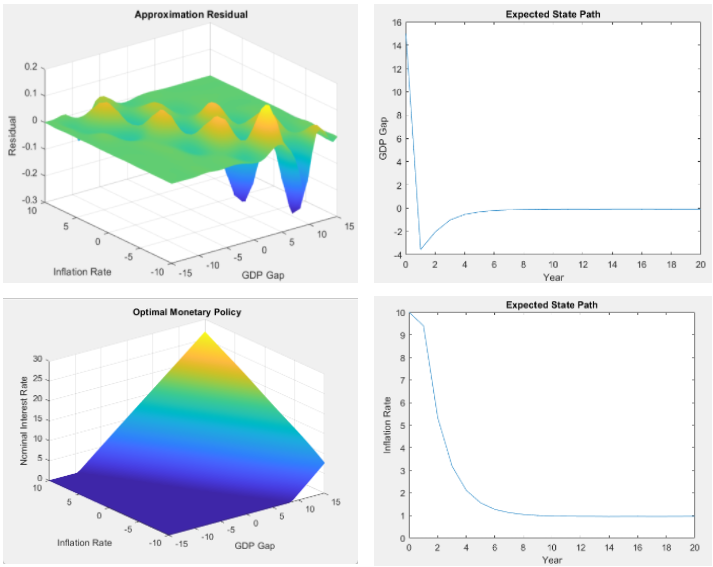
\includegraphics[width=\columnwidth]{img/Optimal_Monetary_Policy/Optimal_Monetary_Policy}
	\caption{Approximation Residuals}
	\label{fig:myf1}
\end{figure}
\begin{figure}
	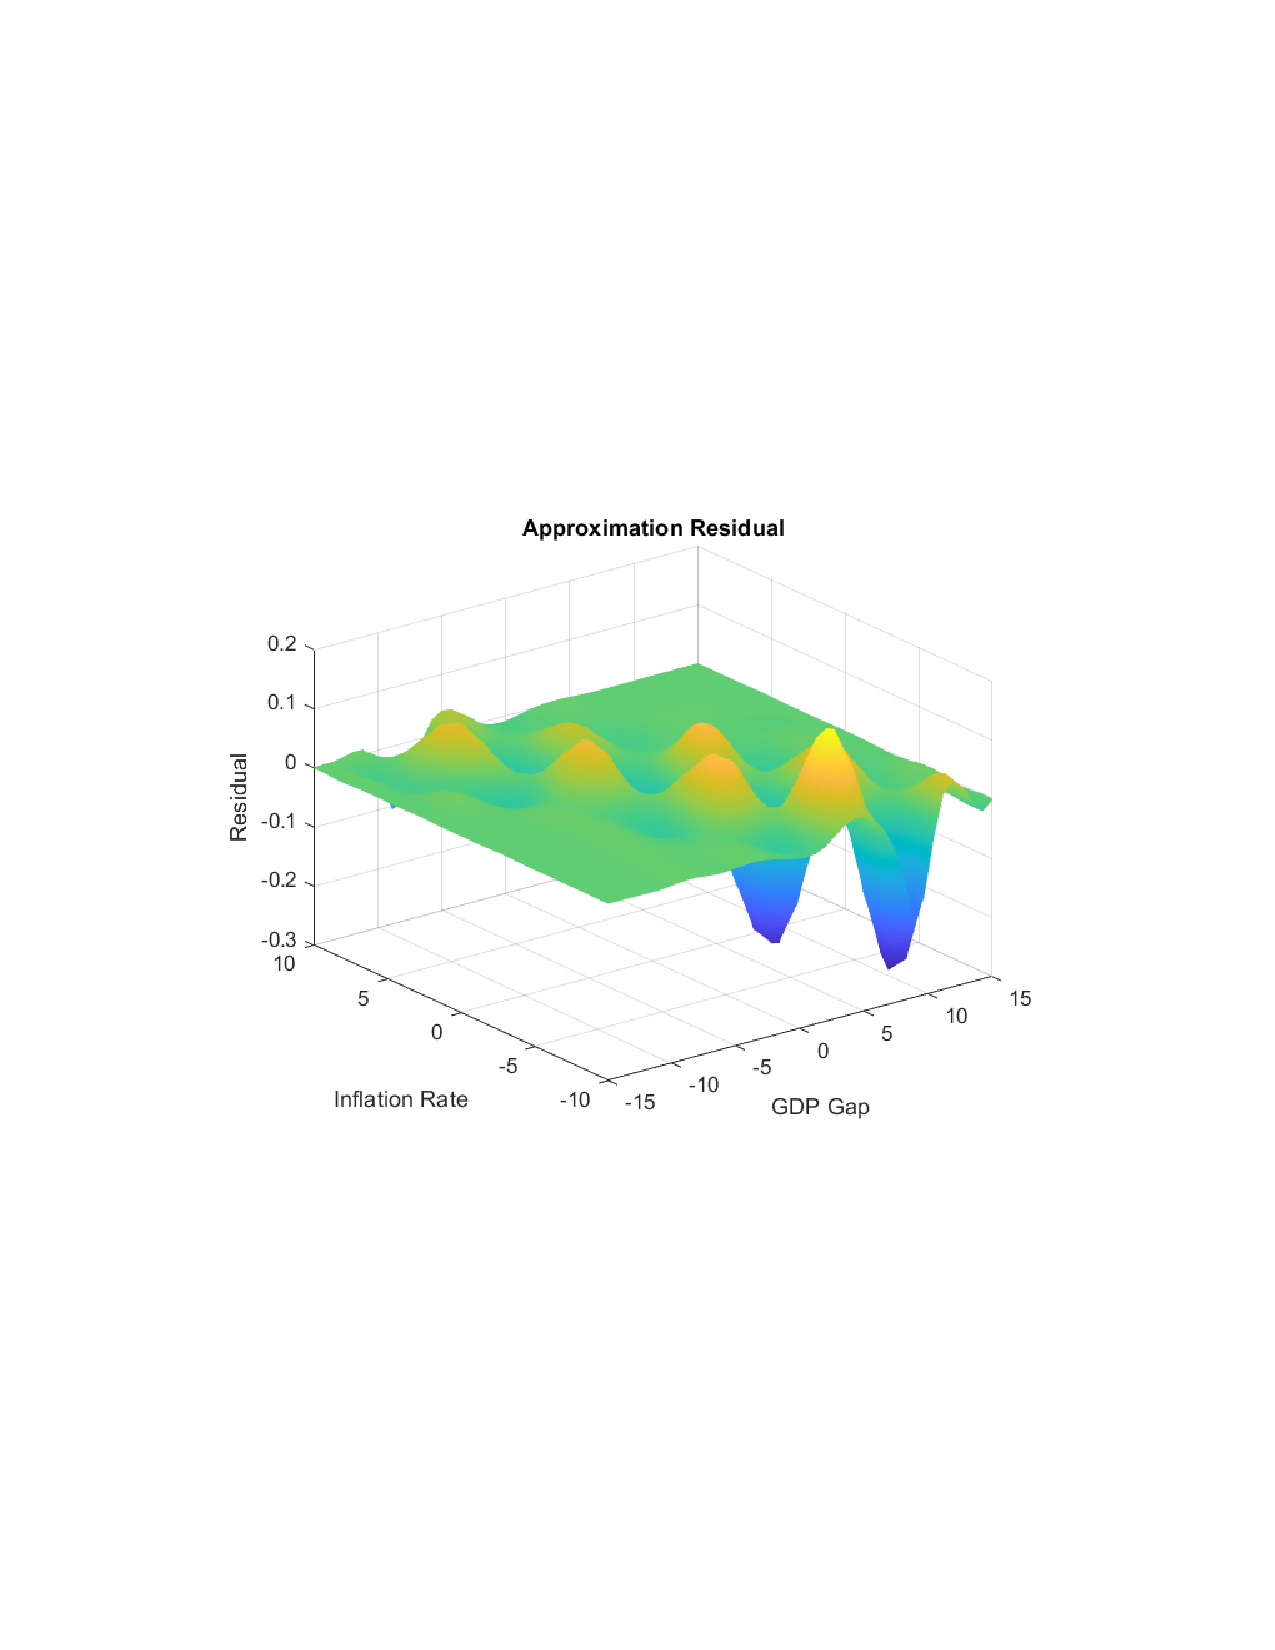
\includegraphics[width=\columnwidth]{img/Optimal_Monetary_Policy/Approximation_Residual}
	\caption{Approximation Residuals}
	\label{fig:myf1}
\end{figure}
\begin{figure}
	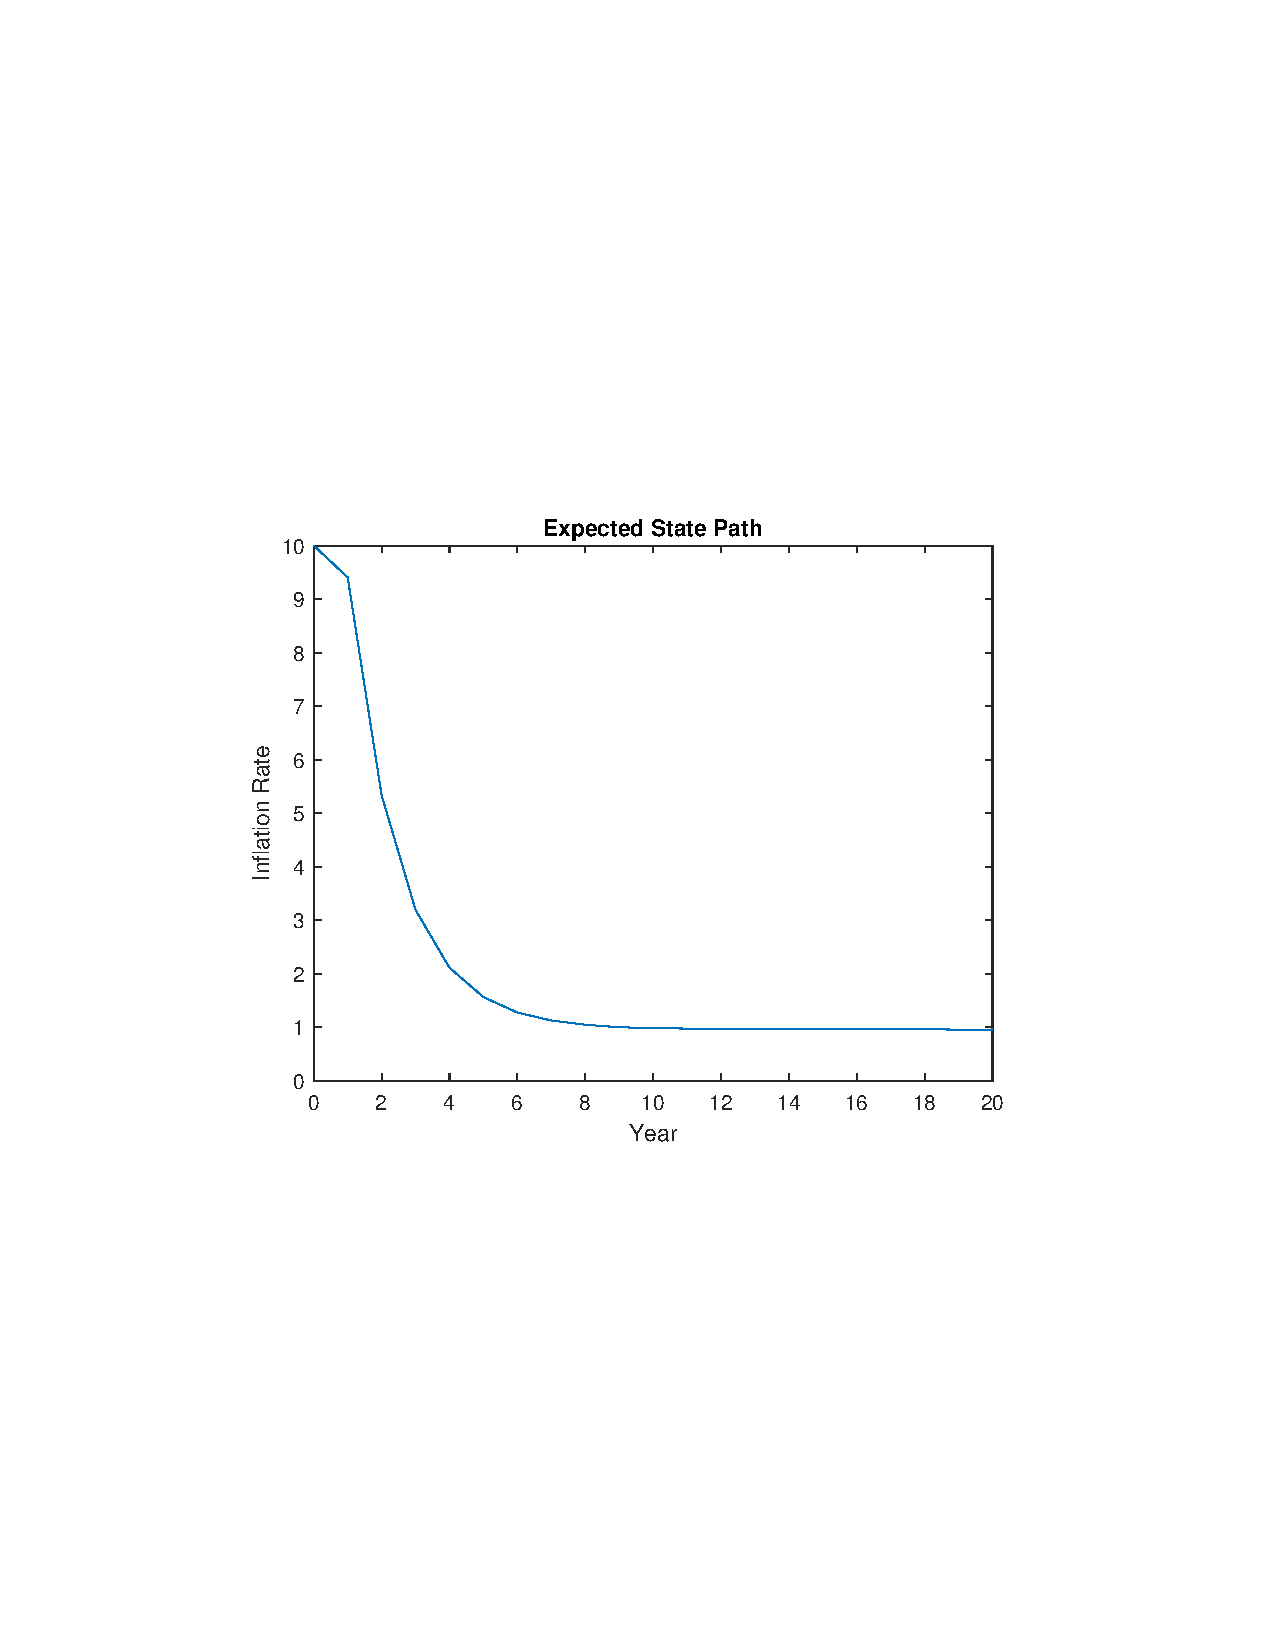
\includegraphics[width=\columnwidth]{img/Optimal_Monetary_Policy/Expected_State_Path_InflationRate}
	\caption{Approximation Residuals}
	\label{fig:myf1}
\end{figure}
\begin{figure}
	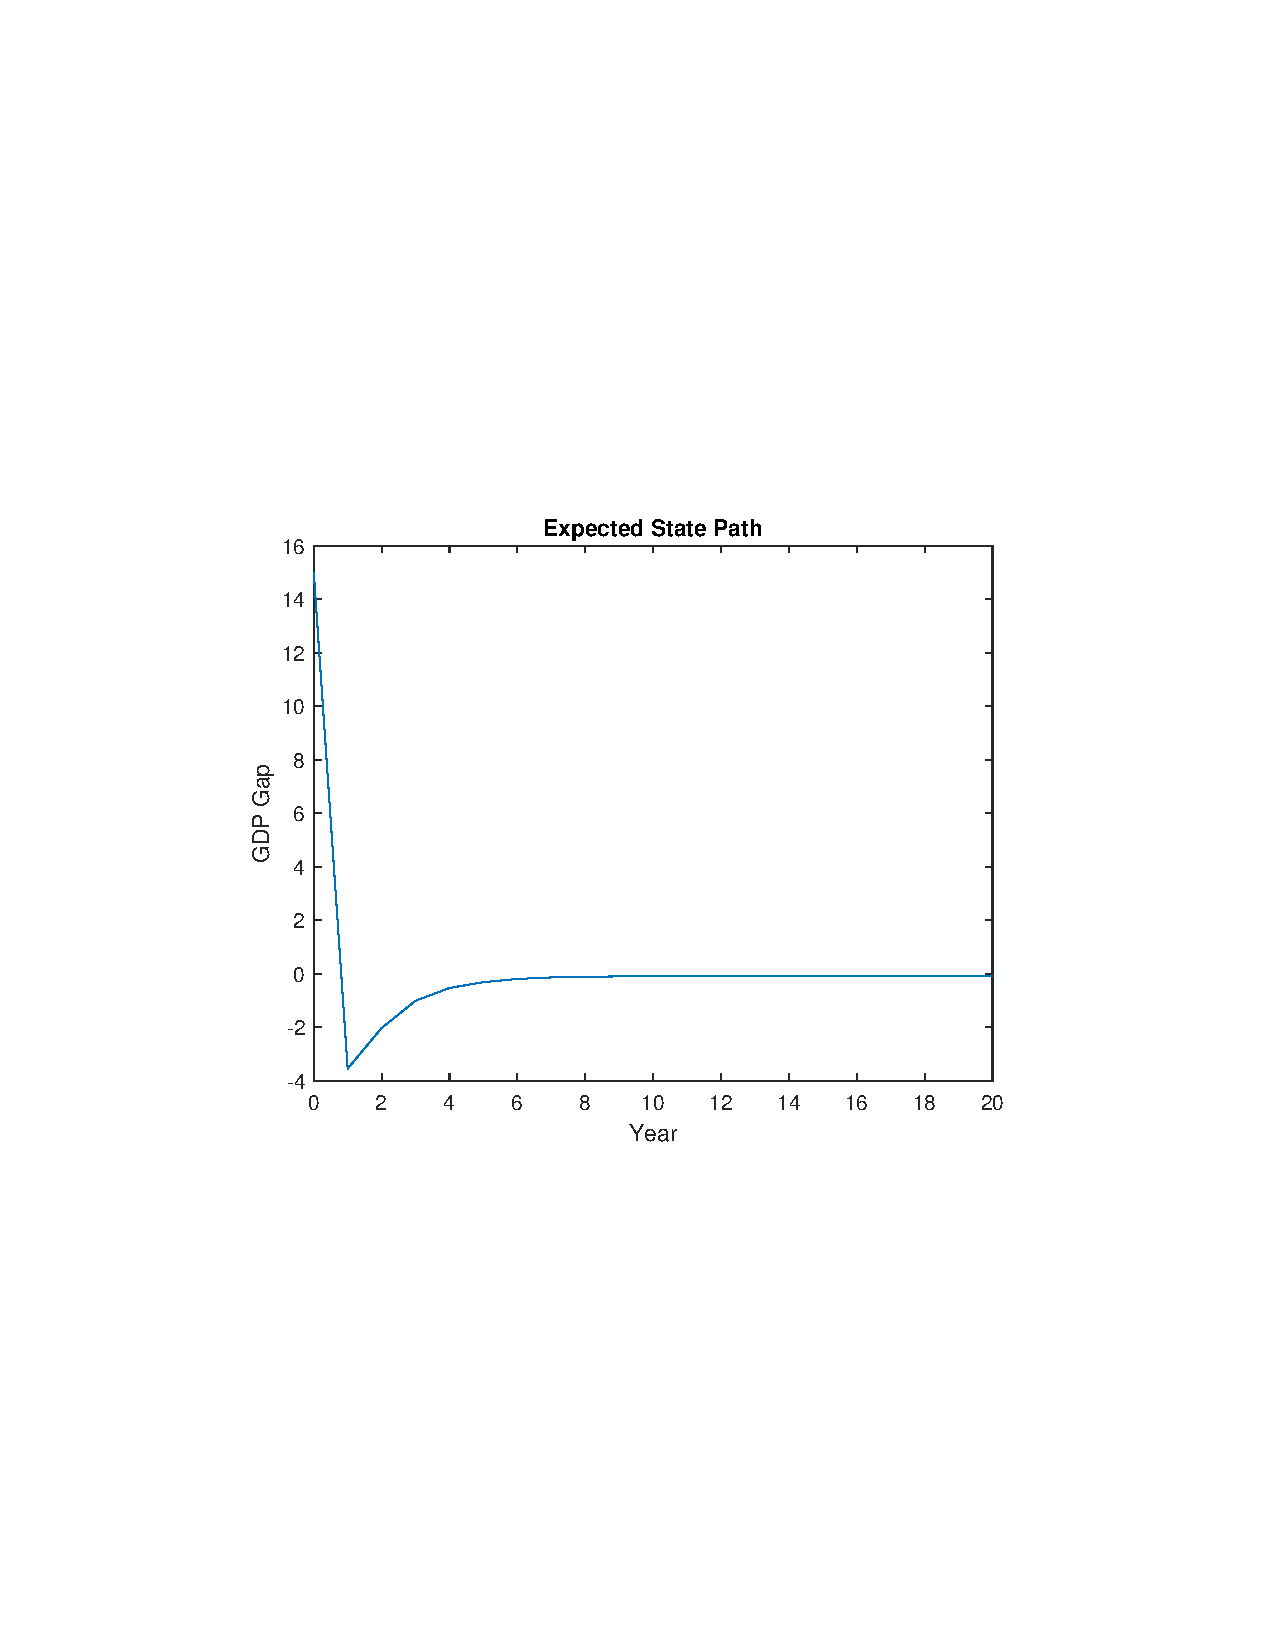
\includegraphics[width=\columnwidth]{img/Optimal_Monetary_Policy/Expected_State_Path_GDP_GAP}
	\caption{Approximation Residuals}
	\label{fig:myf1}
\end{figure}
\end{appendices}
\end{document}